\section{Javascript Testing}
Nachdem eingangs verschiedene allgemeine Testarten und -methodiken aufgeführt wurden, sollen im folgenden konkrete Frameworks für die Programmiersprache Javascript aufgeführt und in Bezug auf diese allgemeinen Ansätze miteinander verglichen werden. Wie in der Einleitung erläutert, wird dabei auch untersucht, ob und wie sich die Tests in Browsern bzw. von einem eigenständigen Javascript-Interpreter ausführen lassen.

\subsection{Modultest-Frameworks}
Zunächst folgen Javascript-Frameworks, mit denen man Modultests schreiben kann.

\subsubsection{JsUnit}
\begin{figure}[!ht]
  \begin{center}
    
\includegraphics[width=3cm]{bilder/jsunit.jpg}
    \caption{Logo von JS-Unit}
    \label{an_tranciver}
  \end{center}
\end{figure}
JsUnit ist das Javascript-Framework der xUnit-Reihe. Es handelt sich also um eine Portierung des von Kent Beck entworfenen Modultest-Frameworks SUnit. Demzufolge bietet sie sowohl die Möglichkeit, Set-Up- und Tear-Down-Methoden, als auch Behauptungen zu formulieren:
\lstinputlisting[language=HTML]{codebeispiele/jsunit.html}
Um den Test-Case auszuführen, bietet JsUnit einen Test-Runner, den man als HTML- Seite in einem beliebigen Browser öffnen kann. In diesem kann man über ein Text-Feld die oben gezeigte Test-Case-Datei referenzieren und ausführen.
\begin{figure}[!ht]
  \begin{center}
    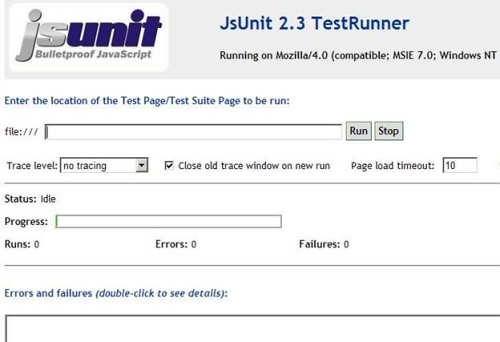
\includegraphics[width=12cm]{bilder/jsunit-testrunner.jpg}
    \caption{JS-Unit Testrunner}
    \label{an_tranciver}
  \end{center}
\end{figure}
JsUnit bietet von Haus aus keine Möglichkeit, den Test-Case in einem Headless- Javascript-Interpreter auszuführen. Dadurch ist eine einfache, automatisierte Ausführung der Tests nicht möglich. Zudem bietet das Framework keine Möglichkeit, die Test-Cases in Test-Suiten zu organisieren. Die Entwicklung von JsUnit wurde inzwischen eingestellt.

\subsubsection{YUI Test}

\subsubsection{Jasmine}

\subsection{Funktionstest-Frameworks}

\subsubsection{Phantom-JS}

\subsubsection{Selenium-Driver}

\subsection{Test Driven Development}

\subsubsection{Browserfernsteuerung}

\subsubsection{Browser-Mocking}

\subsection{Behaviour Driven Development}

\subsection{Continous Integration}

\subsubsection{Karma}

\subsubsection{SauceLabs}

